
%% bare_jrnl.tex
%% V1.3
%% 2007/01/11
%% by Michael Shell
%% see http://www.michaelshell.org/
%% for current contact information.
%%
%% This is a skeleton file demonstrating the use of IEEEtran.cls
%% (requires IEEEtran.cls version 1.7 or later) with an IEEE journal paper.
%%
%% Support sites:
%% http://www.michaelshell.org/tex/ieeetran/
%% http://www.ctan.org/tex-archive/macros/latex/contrib/IEEEtran/
%% and
%% http://www.ieee.org/



% *** Authors should verify (and, if needed, correct) their LaTeX system  ***
% *** with the testflow diagnostic prior to trusting their LaTeX platform ***
% *** with production work. IEEE's font choices can trigger bugs that do  ***
% *** not appear when using other class files.                            ***
% The testflow support page is at:
% http://www.michaelshell.org/tex/testflow/


%%*************************************************************************
%% Legal Notice:
%% This code is offered as-is without any warranty either expressed or
%% implied; without even the implied warranty of MERCHANTABILITY or
%% FITNESS FOR A PARTICULAR PURPOSE! 
%% User assumes all risk.
%% In no event shall IEEE or any contributor to this code be liable for
%% any damages or losses, including, but not limited to, incidental,
%% consequential, or any other damages, resulting from the use or misuse
%% of any information contained here.
%%
%% All comments are the opinions of their respective authors and are not
%% necessarily endorsed by the IEEE.
%%
%% This work is distributed under the LaTeX Project Public License (LPPL)
%% ( http://www.latex-project.org/ ) version 1.3, and may be freely used,
%% distributed and modified. A copy of the LPPL, version 1.3, is included
%% in the base LaTeX documentation of all distributions of LaTeX released
%% 2003/12/01 or later.
%% Retain all contribution notices and credits.
%% ** Modified files should be clearly indicated as such, including  **
%% ** renaming them and changing author support contact information. **
%%
%% File list of work: IEEEtran.cls, IEEEtran_HOWTO.pdf, bare_adv.tex,
%%                    bare_conf.tex, bare_jrnl.tex, bare_jrnl_compsoc.tex
%%*************************************************************************

% Note that the a4paper option is mainly intended so that authors in
% countries using A4 can easily print to A4 and see how their papers will
% look in print - the typesetting of the document will not typically be
% affected with changes in paper size (but the bottom and side margins will).
% Use the testflow package mentioned above to verify correct handling of
% both paper sizes by the user's LaTeX system.
%
% Also note that the "draftcls" or "draftclsnofoot", not "draft", option
% should be used if it is desired that the figures are to be displayed in
% draft mode.
%
\documentclass[journal]{IEEEtran}
\usepackage{blindtext}
\usepackage{graphicx}

% Some very useful LaTeX packages include:
% (uncomment the ones you want to load)


% *** MISC UTILITY PACKAGES ***
%
%\usepackage{ifpdf}
% Heiko Oberdiek's ifpdf.sty is very useful if you need conditional
% compilation based on whether the output is pdf or dvi.
% usage:
% \ifpdf
%   % pdf code
% \else
%   % dvi code
% \fi
% The latest version of ifpdf.sty can be obtained from:
% http://www.ctan.org/tex-archive/macros/latex/contrib/oberdiek/
% Also, note that IEEEtran.cls V1.7 and later provides a builtin
% \ifCLASSINFOpdf conditional that works the same way.
% When switching from latex to pdflatex and vice-versa, the compiler may
% have to be run twice to clear warning/error messages.






% *** CITATION PACKAGES ***
%
%\usepackage{cite}
% cite.sty was written by Donald Arseneau
% V1.6 and later of IEEEtran pre-defines the format of the cite.sty package
% \cite{} output to follow that of IEEE. Loading the cite package will
% result in citation numbers being automatically sorted and properly
% "compressed/ranged". e.g., [1], [9], [2], [7], [5], [6] without using
% cite.sty will become [1], [2], [5]--[7], [9] using cite.sty. cite.sty's
% \cite will automatically add leading space, if needed. Use cite.sty's
% noadjust option (cite.sty V3.8 and later) if you want to turn this off.
% cite.sty is already installed on most LaTeX systems. Be sure and use
% version 4.0 (2003-05-27) and later if using hyperref.sty. cite.sty does
% not currently provide for hyperlinked citations.
% The latest version can be obtained at:
% http://www.ctan.org/tex-archive/macros/latex/contrib/cite/
% The documentation is contained in the cite.sty file itself.






% *** GRAPHICS RELATED PACKAGES ***
%
\ifCLASSINFOpdf
  % \usepackage[pdftex]{graphicx}
  % declare the path(s) where your graphic files are
  % \graphicspath{{../pdf/}{../jpeg/}}
  % and their extensions so you won't have to specify these with
  % every instance of \includegraphics
  % \DeclareGraphicsExtensions{.pdf,.jpeg,.png}
\else
  % or other class option (dvipsone, dvipdf, if not using dvips). graphicx
  % will default to the driver specified in the system graphics.cfg if no
  % driver is specified.
  % \usepackage[dvips]{graphicx}
  % declare the path(s) where your graphic files are
  % \graphicspath{{../eps/}}
  % and their extensions so you won't have to specify these with
  % every instance of \includegraphics
  % \DeclareGraphicsExtensions{.eps}
\fi
% graphicx was written by David Carlisle and Sebastian Rahtz. It is
% required if you want graphics, photos, etc. graphicx.sty is already
% installed on most LaTeX systems. The latest version and documentation can
% be obtained at: 
% http://www.ctan.org/tex-archive/macros/latex/required/graphics/
% Another good source of documentation is "Using Imported Graphics in
% LaTeX2e" by Keith Reckdahl which can be found as epslatex.ps or
% epslatex.pdf at: http://www.ctan.org/tex-archive/info/
%
% latex, and pdflatex in dvi mode, support graphics in encapsulated
% postscript (.eps) format. pdflatex in pdf mode supports graphics
% in .pdf, .jpeg, .png and .mps (metapost) formats. Users should ensure
% that all non-photo figures use a vector format (.eps, .pdf, .mps) and
% not a bitmapped formats (.jpeg, .png). IEEE frowns on bitmapped formats
% which can result in "jaggedy"/blurry rendering of lines and letters as
% well as large increases in file sizes.
%
% You can find documentation about the pdfTeX application at:
% http://www.tug.org/applications/pdftex





% *** MATH PACKAGES ***
%
%\usepackage[cmex10]{amsmath}
% A popular package from the American Mathematical Society that provides
% many useful and powerful commands for dealing with mathematics. If using
% it, be sure to load this package with the cmex10 option to ensure that
% only type 1 fonts will utilized at all point sizes. Without this option,
% it is possible that some math symbols, particularly those within
% footnotes, will be rendered in bitmap form which will result in a
% document that can not be IEEE Xplore compliant!
%
% Also, note that the amsmath package sets \interdisplaylinepenalty to 10000
% thus preventing page breaks from occurring within multiline equations. Use:
%\interdisplaylinepenalty=2500
% after loading amsmath to restore such page breaks as IEEEtran.cls normally
% does. amsmath.sty is already installed on most LaTeX systems. The latest
% version and documentation can be obtained at:
% http://www.ctan.org/tex-archive/macros/latex/required/amslatex/math/





% *** SPECIALIZED LIST PACKAGES ***
%
%\usepackage{algorithmic}
% algorithmic.sty was written by Peter Williams and Rogerio Brito.
% This package provides an algorithmic environment fo describing algorithms.
% You can use the algorithmic environment in-text or within a figure
% environment to provide for a floating algorithm. Do NOT use the algorithm
% floating environment provided by algorithm.sty (by the same authors) or
% algorithm2e.sty (by Christophe Fiorio) as IEEE does not use dedicated
% algorithm float types and packages that provide these will not provide
% correct IEEE style captions. The latest version and documentation of
% algorithmic.sty can be obtained at:
% http://www.ctan.org/tex-archive/macros/latex/contrib/algorithms/
% There is also a support site at:
% http://algorithms.berlios.de/index.html
% Also of interest may be the (relatively newer and more customizable)
% algorithmicx.sty package by Szasz Janos:
% http://www.ctan.org/tex-archive/macros/latex/contrib/algorithmicx/




% *** ALIGNMENT PACKAGES ***
%
%\usepackage{array}
% Frank Mittelbach's and David Carlisle's array.sty patches and improves
% the standard LaTeX2e array and tabular environments to provide better
% appearance and additional user controls. As the default LaTeX2e table
% generation code is lacking to the point of almost being broken with
% respect to the quality of the end results, all users are strongly
% advised to use an enhanced (at the very least that provided by array.sty)
% set of table tools. array.sty is already installed on most systems. The
% latest version and documentation can be obtained at:
% http://www.ctan.org/tex-archive/macros/latex/required/tools/


%\usepackage{mdwmath}
%\usepackage{mdwtab}
% Also highly recommended is Mark Wooding's extremely powerful MDW tools,
% especially mdwmath.sty and mdwtab.sty which are used to format equations
% and tables, respectively. The MDWtools set is already installed on most
% LaTeX systems. The lastest version and documentation is available at:
% http://www.ctan.org/tex-archive/macros/latex/contrib/mdwtools/


% IEEEtran contains the IEEEeqnarray family of commands that can be used to
% generate multiline equations as well as matrices, tables, etc., of high
% quality.


%\usepackage{eqparbox}
% Also of notable interest is Scott Pakin's eqparbox package for creating
% (automatically sized) equal width boxes - aka "natural width parboxes".
% Available at:
% http://www.ctan.org/tex-archive/macros/latex/contrib/eqparbox/





% *** SUBFIGURE PACKAGES ***
%\usepackage[tight,footnotesize]{subfigure}
% subfigure.sty was written by Steven Douglas Cochran. This package makes it
% easy to put subfigures in your figures. e.g., "Figure 1a and 1b". For IEEE
% work, it is a good idea to load it with the tight package option to reduce
% the amount of white space around the subfigures. subfigure.sty is already
% installed on most LaTeX systems. The latest version and documentation can
% be obtained at:
% http://www.ctan.org/tex-archive/obsolete/macros/latex/contrib/subfigure/
% subfigure.sty has been superceeded by subfig.sty.



%\usepackage[caption=false]{caption}
%\usepackage[font=footnotesize]{subfig}
% subfig.sty, also written by Steven Douglas Cochran, is the modern
% replacement for subfigure.sty. However, subfig.sty requires and
% automatically loads Axel Sommerfeldt's caption.sty which will override
% IEEEtran.cls handling of captions and this will result in nonIEEE style
% figure/table captions. To prevent this problem, be sure and preload
% caption.sty with its "caption=false" package option. This is will preserve
% IEEEtran.cls handing of captions. Version 1.3 (2005/06/28) and later 
% (recommended due to many improvements over 1.2) of subfig.sty supports
% the caption=false option directly:
%\usepackage[caption=false,font=footnotesize]{subfig}
%
% The latest version and documentation can be obtained at:
% http://www.ctan.org/tex-archive/macros/latex/contrib/subfig/
% The latest version and documentation of caption.sty can be obtained at:
% http://www.ctan.org/tex-archive/macros/latex/contrib/caption/




% *** FLOAT PACKAGES ***
%
%\usepackage{fixltx2e}
% fixltx2e, the successor to the earlier fix2col.sty, was written by
% Frank Mittelbach and David Carlisle. This package corrects a few problems
% in the LaTeX2e kernel, the most notable of which is that in current
% LaTeX2e releases, the ordering of single and double column floats is not
% guaranteed to be preserved. Thus, an unpatched LaTeX2e can allow a
% single column figure to be placed prior to an earlier double column
% figure. The latest version and documentation can be found at:
% http://www.ctan.org/tex-archive/macros/latex/base/



%\usepackage{stfloats}
% stfloats.sty was written by Sigitas Tolusis. This package gives LaTeX2e
% the ability to do double column floats at the bottom of the page as well
% as the top. (e.g., "\begin{figure*}[!b]" is not normally possible in
% LaTeX2e). It also provides a command:
%\fnbelowfloat
% to enable the placement of footnotes below bottom floats (the standard
% LaTeX2e kernel puts them above bottom floats). This is an invasive package
% which rewrites many portions of the LaTeX2e float routines. It may not work
% with other packages that modify the LaTeX2e float routines. The latest
% version and documentation can be obtained at:
% http://www.ctan.org/tex-archive/macros/latex/contrib/sttools/
% Documentation is contained in the stfloats.sty comments as well as in the
% presfull.pdf file. Do not use the stfloats baselinefloat ability as IEEE
% does not allow \baselineskip to stretch. Authors submitting work to the
% IEEE should note that IEEE rarely uses double column equations and
% that authors should try to avoid such use. Do not be tempted to use the
% cuted.sty or midfloat.sty packages (also by Sigitas Tolusis) as IEEE does
% not format its papers in such ways.


%\ifCLASSOPTIONcaptionsoff
%  \usepackage[nomarkers]{endfloat}
% \let\MYoriglatexcaption\caption
% \renewcommand{\caption}[2][\relax]{\MYoriglatexcaption[#2]{#2}}
%\fi
% endfloat.sty was written by James Darrell McCauley and Jeff Goldberg.
% This package may be useful when used in conjunction with IEEEtran.cls'
% captionsoff option. Some IEEE journals/societies require that submissions
% have lists of figures/tables at the end of the paper and that
% figures/tables without any captions are placed on a page by themselves at
% the end of the document. If needed, the draftcls IEEEtran class option or
% \CLASSINPUTbaselinestretch interface can be used to increase the line
% spacing as well. Be sure and use the nomarkers option of endfloat to
% prevent endfloat from "marking" where the figures would have been placed
% in the text. The two hack lines of code above are a slight modification of
% that suggested by in the endfloat docs (section 8.3.1) to ensure that
% the full captions always appear in the list of figures/tables - even if
% the user used the short optional argument of \caption[]{}.
% IEEE papers do not typically make use of \caption[]'s optional argument,
% so this should not be an issue. A similar trick can be used to disable
% captions of packages such as subfig.sty that lack options to turn off
% the subcaptions:
% For subfig.sty:
% \let\MYorigsubfloat\subfloat
% \renewcommand{\subfloat}[2][\relax]{\MYorigsubfloat[]{#2}}
% For subfigure.sty:
% \let\MYorigsubfigure\subfigure
% \renewcommand{\subfigure}[2][\relax]{\MYorigsubfigure[]{#2}}
% However, the above trick will not work if both optional arguments of
% the \subfloat/subfig command are used. Furthermore, there needs to be a
% description of each subfigure *somewhere* and endfloat does not add
% subfigure captions to its list of figures. Thus, the best approach is to
% avoid the use of subfigure captions (many IEEE journals avoid them anyway)
% and instead reference/explain all the subfigures within the main caption.
% The latest version of endfloat.sty and its documentation can obtained at:
% http://www.ctan.org/tex-archive/macros/latex/contrib/endfloat/
%
% The IEEEtran \ifCLASSOPTIONcaptionsoff conditional can also be used
% later in the document, say, to conditionally put the References on a 
% page by themselves.





% *** PDF, URL AND HYPERLINK PACKAGES ***
%
%\usepackage{url}
% url.sty was written by Donald Arseneau. It provides better support for
% handling and breaking URLs. url.sty is already installed on most LaTeX
% systems. The latest version can be obtained at:
% http://www.ctan.org/tex-archive/macros/latex/contrib/misc/
% Read the url.sty source comments for usage information. Basically,
% \url{my_url_here}.

% *** Do not adjust lengths that control margins, column widths, etc. ***
% *** Do not use packages that alter fonts (such as pslatex).         ***
% There should be no need to do such things with IEEEtran.cls V1.6 and later.
% (Unless specifically asked to do so by the journal or conference you plan
% to submit to, of course. )

\usepackage{amsfonts}
\usepackage{amsmath}
\usepackage{amsthm}
\usepackage{float}
\usepackage{graphicx}
\usepackage{hyperref}

% correct bad hyphenation here
\begin{document}
\title{Upon the Deanonymization of Bitcoin Transactions}
\author{Yash Patel, Matt Weinberg}

\markboth{MAT Senior Thesis 2018}%
{Shell \MakeLowercase{\textit{et al.}}: Bare Demo of IEEEtran.cls for Journals}
\maketitle

\begin{abstract}
\end{abstract}

\section{Introduction}
Bitcoin, previously relegated as a technology residing in the niche of only the most technologically competent of computer scientists, has emerged into the mainstream public in an enormous way. Ever since its explosive rise over the past year, technologists and investors both have sought to understand and exploit its technical limits. As illustrated in Figure \ref{fig:BTC_price}, speculation on the asset of Bitcoin has become an undeniable sector of the modern technology world, especially when viewed from those outside of it. While current speculations are high, many investors and technologists both struggle to understand the fundamental use case of Bitcoin and its underlying technology: blockchain. The speculative bubble is largely the product of vacuous interest pooling into an asset of misunderstood potential, paralleling the financial bubble surrounding the dot-com bubble. 

\begin{figure}
    \label{fig:BTC_price}
    \centering
    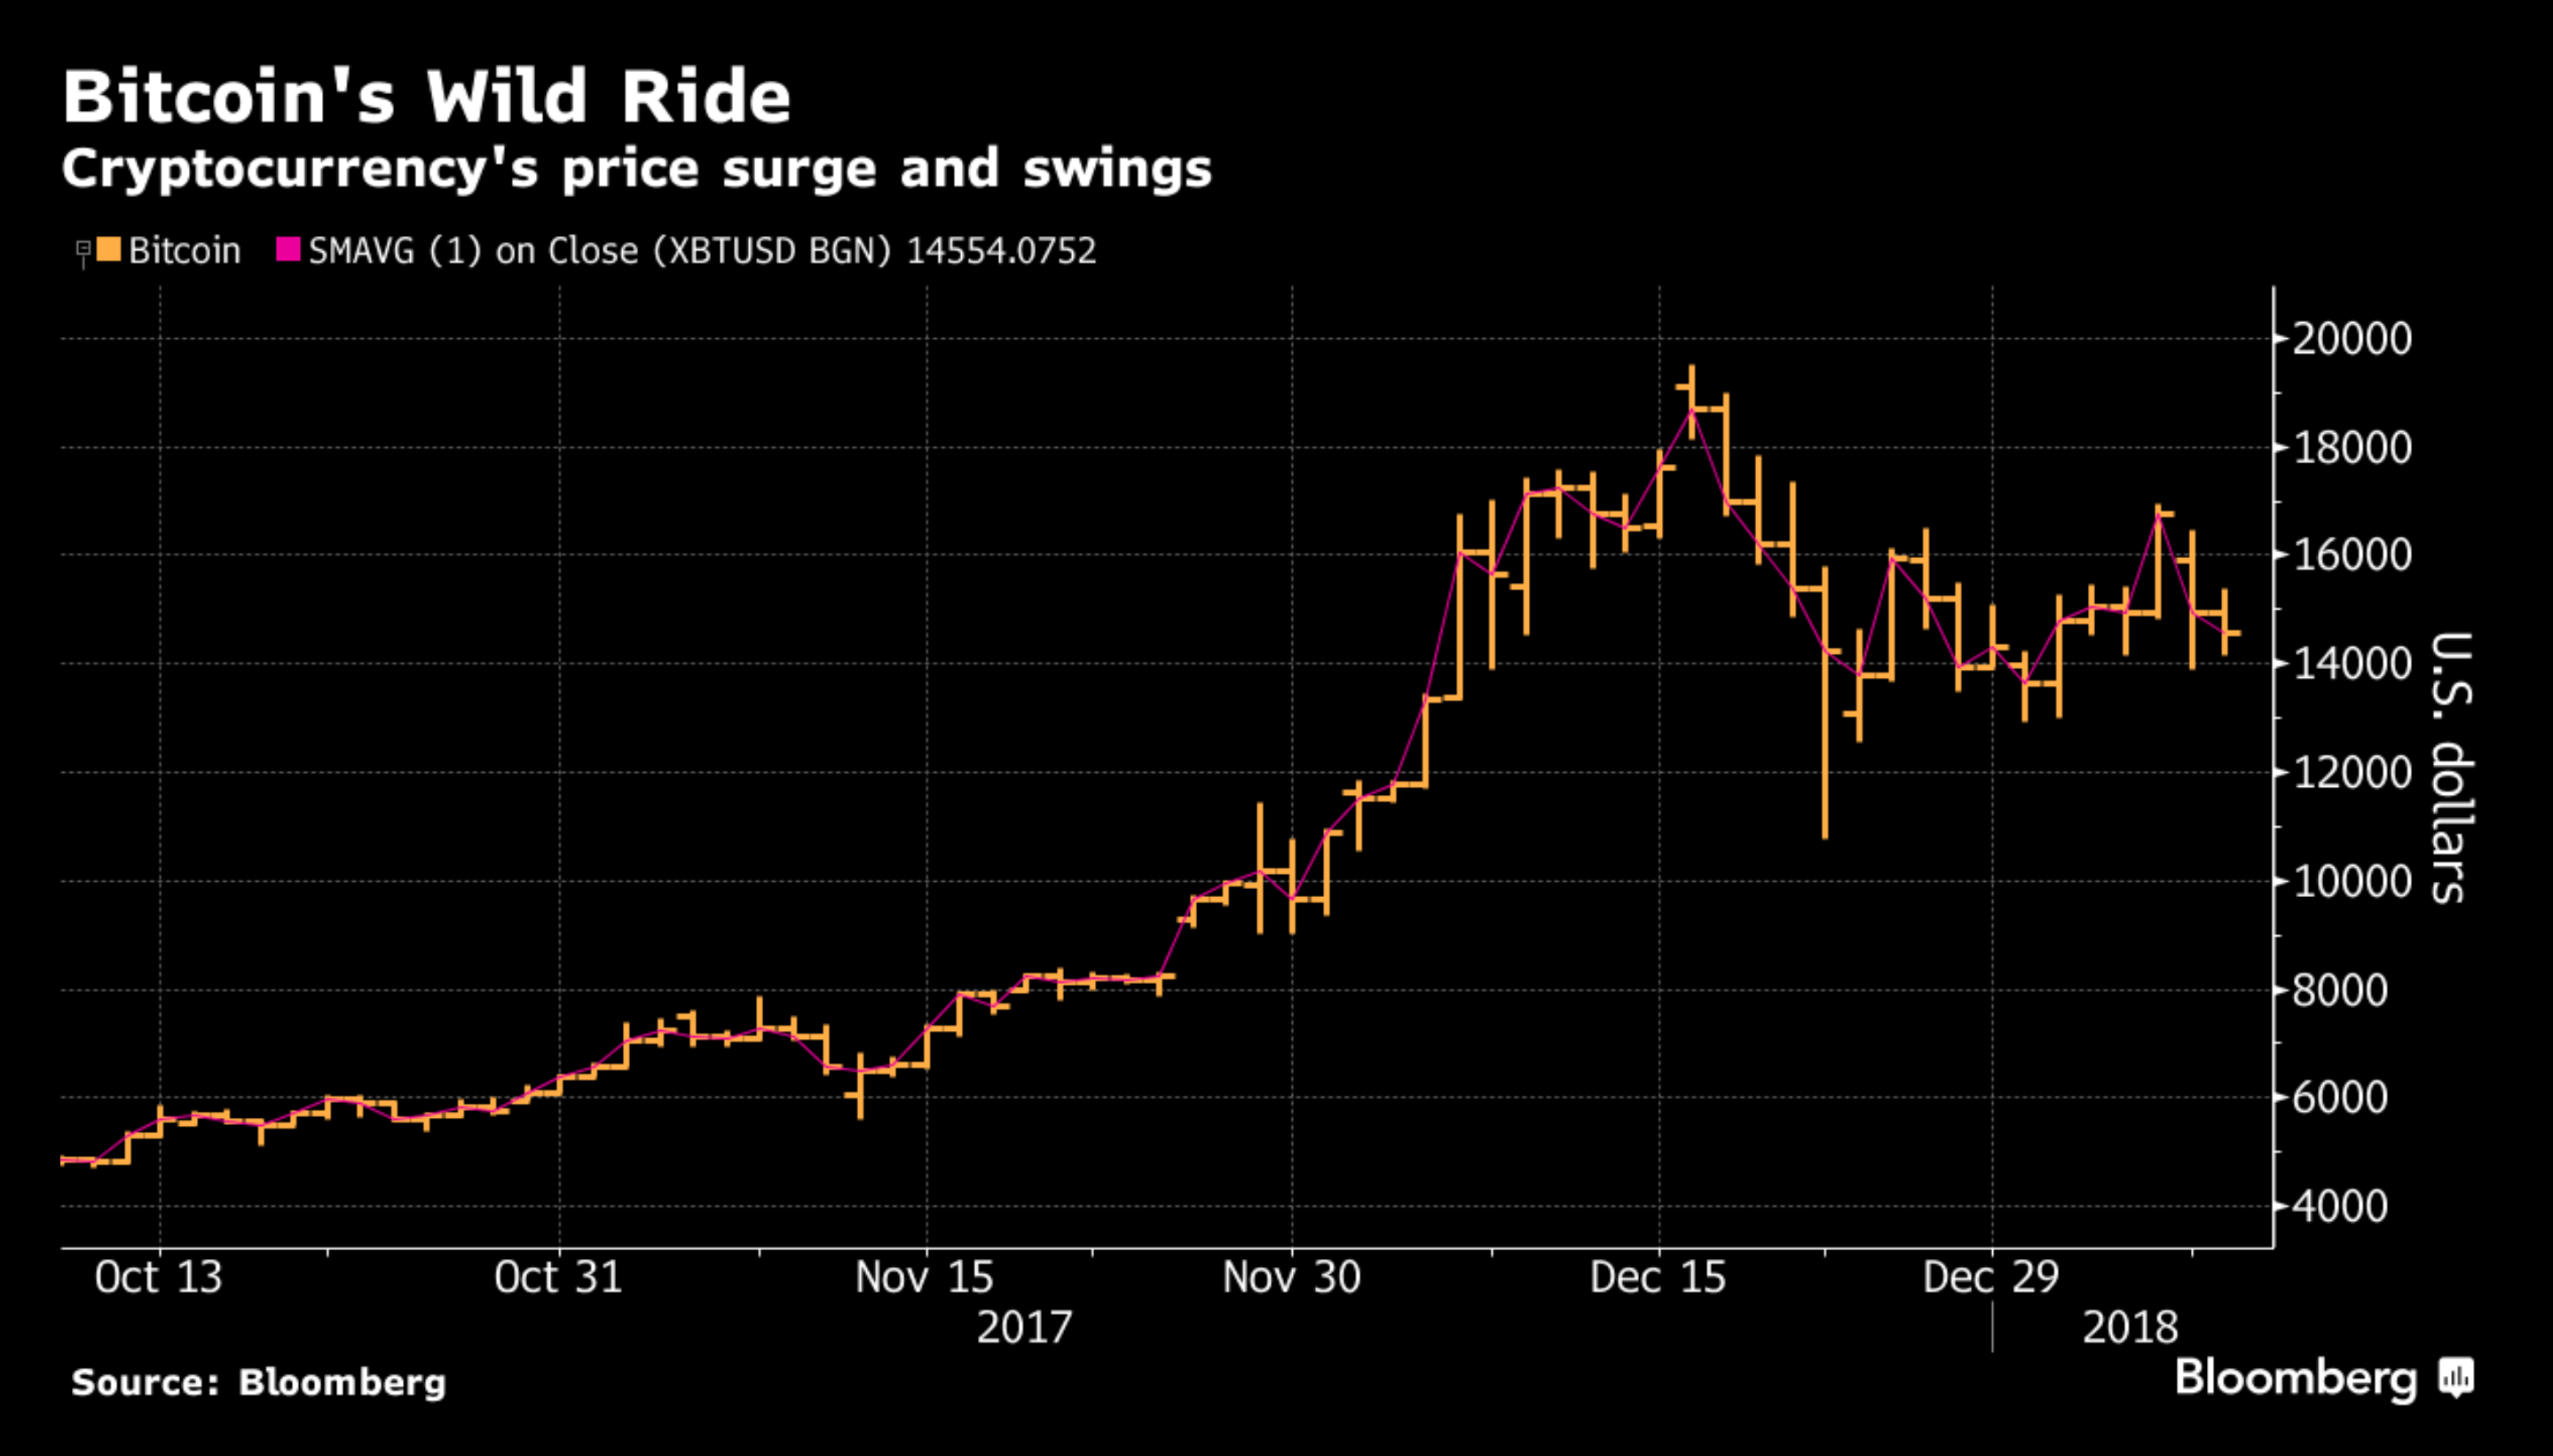
\includegraphics[width=0.4\textwidth]{BTC_price.png}
    \caption{The price of one Bitcoin, as marked by Bloomberg. While technologists saw its promise many years prior, Bitcoin's rise in popularity in the general public has led to exponential speculative interest \cite{goldman}.}
\end{figure}

Prior to further discussing Bitcoin's use cases as a whole, it serves a purpose to understand both the technology and underlying technology first. Briefly, Bitcoin is a cryptocurrency, by which we mean a ``digital unit of exchange that is not backed by a government-issued legal tender" \cite{virtual}. The blockchain technology underpinning Bitcoin and other cryptocurrencies, as illustrated in Figure \ref{fig:blockchain}, is ``a solution to the double-spending problem using a peer-to-peer distributed timestamp server to generate computational proof of the chronological order of transactions. The system is secure as long as honest nodes collectively control more CPU power than any cooperating group of attacker nodes" \cite{bitcoin}. Described plainly, blockchain seeks to solve a technical problem, namely that of achieving consensus in a distributed system while preventing double-spending of the asset being exchanged, i.e. arbitrating exchange of a common asset without the need of a trusted central authority. Bitcoin happens to be one such asset, but there now exist many others, each building further layers of properties to serve their own purposes.

\begin{figure}
    \label{fig:blockchain}
    \centering
    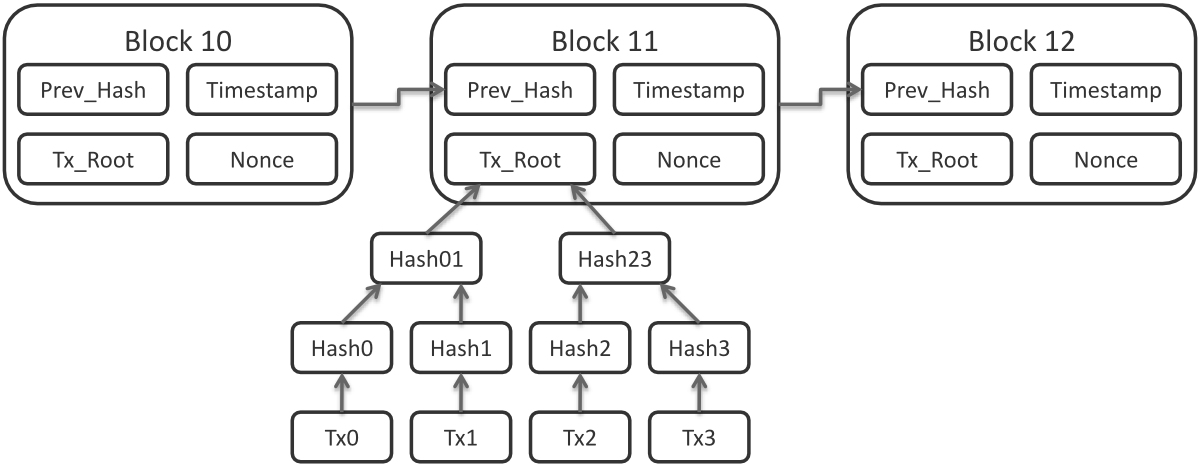
\includegraphics[width=0.4\textwidth]{blockchain.png}
    \caption{Blockchain, the underlying technology behind Bitcoin and all other cryptocurrencies, is simply a data structure consisting of an extended linked list of hash pointers with metadata. These pieces of metadata, in addition to carrying the actual BTC information of interest, more importantly serve as a piece of data that can be used for efficient verification of double-spending in a distributed system \cite{blockchain-img}.}
\end{figure}

Simply viewed from this perspective, there appears to be nothing inherent in the association of Bitcoin with privacy. This aspect of blockchain and BTC largely arises from social concerns. Specifically, given that the blockchain ledger is available in a distributed setting, all transactions are publicly visible. 

Bitcoin, by contrast, is designed with pseudonymous identities. Account numbers are public keys of a specific asymmetric encryption system \cite{laundering}.

Returning to the topic of interest, many of the use cases emerged surrounding Bitcoin and the cryptocurrency space in general reside in the realms of piracy and illicit activity, into which we briefly delve. 


This includes Bitcoin, a decentralized cryptographic currency which emerged over the past three years and has been regarded with suspicion for its allegedly anonymous and irreversible transactions, its popularity in underground markets, and its association with several cases of investment fraud \cite{laundering}.

anonymous online market very often specialize in ``black market" goods, such as pornography, weapons or narcotics. Silk Road is one such anonymous online market \cite{silk}.

Silk Road only supports Bitcoin (BTC, [30]) as a trading currency. Bitcoin is a peer-to-peer, distributed payment system that supports verifiable transactions without the need for a central third-part \cite{silk}.

Comparing the two numbers shows that Silk Road transactions correspond to about 4.5\% of all transactions occurring in exchange \cite{silk}.

regulation of virtual currencies, cybercrimes and payment systems, darknets, Tor and the “deep web,” Bitcoin; Liberty Reserve, Silk Road, and Mt. Gox. Virtual currencies have quickly become a reality, gaining significant traction in a very short period of time, and are evolving rapidly \cite{virtual-currency}.

present particularly difficult law enforcement challenges because of their ability to transcend national borders in the fraction of a second, unique jurisdictional issues and anonymity due to encryption. Due primarily to their anonymity, virtual currencies have been linked to numerous types of crimes, including facilitating marketplaces for: assassins, attacks on businesses, the exploitation of children (including pornography), corporate espionage, counterfeit currencies, drugs, fake IDs and passports, high yield investment schemes (Ponzi schemes and other financial frauds), sexual exploitation, stolen credit cards and credit card numbers, and weapons \cite{virtual-currency}. 

The outline of this paper is, therefore, as follows:
\begin{itemize}
    \item Section \ref{background}: Covers through the major technical topics of interest that are to be used in the remainder of the paper. Most of the findings presented through this section entail a literature review of well-known works in their respective fields, although occasional novel material is presented when appropriate for sake of organization. We further note that a majority of figures presented through this section entail those catered from previous research endeavors.
    \item Section \ref{methodology}: Walks through the structure of the experiments that were written and conducted. The code is freely available at: \url{https://github.com/yashpatel5400/anonychain}. We further provide the specifics of the expected structure of results from each experiment.
    \item Section \ref{results}: Presents the results of the experiments laid of in the previous section, largely in the form of graphs when appropriate and tables otherwise.
    \item Section \ref{discussion}: Discusses the main takeaways from the graphical results as they relate to the research problem posed above. Specifically, these discussions will pointedly answer the extent to which spectral clustering can be used for deanonymizing Bitcoin transactions.
    \item Section \ref{conclusion}: Provide follow-up research ideas that could be pursued should readers feel inspired and interested in furthering the research conducted herein.
\end{itemize}

\section{Background}\label{background}

\section{Methodology}\label{methodology}

\section{Results}\label{results}

\section{Discussion}\label{discussion}

\section{Conclusion}\label{conclusion}

\newpage
\begin{thebibliography}{1}
\bibitem{data-stream} Aggarwal, Charu C., et al. ``A Framework for Clustering Evolving Data Streams." Proceedings 2003 VLDB Conference, 2003, pp. 81–92., doi:10.1016/b978-012722442-8/50016-1.
\bibitem{spectral-sparse} Batson, Joshua, et al. ``Spectral Sparsification of Graphs." Communications of the ACM, vol. 56, no. 8, 2013, p. 87., doi:10.1145/2492007.2492029.
\bibitem{coarsening} Chevalier, Cedric, and Ilya Safro. ``Comparison of Coarsening Schemes for Multilevel Graph Partitioning." Lecture Notes in Computer Science Learning and Intelligent Optimization, 2009, pp. 191–205., doi:10.1007/978-3-642-11169-3\_14.
\bibitem{evolutionary-temporal} Chi, Yun, et al. ``Evolutionary Spectral Clustering by Incorporating Temporal Smoothness." Proceedings of the 13th ACM SIGKDD International Conference on Knowledge Discovery and Data Mining - KDD '07, 2007, doi:10.1145/1281192.1281212.
\bibitem{silk} Christin, Nicolas. ``Traveling the Silk Road: A Measurement of a Large Anonymous Online Marketplace." 2012, doi:10.21236/ada579383.
\bibitem{scikit} ``Clustering." Scikit-Learn, scikit-learn.org/stable/modules/clustering.html.
\bibitem{coinjoin} ``CoinJoin: Bitcoin Privacy for the Real World." Bitcoin Talk, 22 Aug. 2013, bitcointalk.org/index.php?topic=279249.0.
\bibitem{dbscan} Daszykowski, M., and B. Walczak. ``Density-Based Clustering Methods." Comprehensive Chemometrics, 2009, pp. 635–654., doi:10.1016/b978-044452701-1.00067-3.
\bibitem{eigen-update} Dhanjal, Charanpal, et al. ``Efficient Eigen-Updating for Spectral Graph Clustering." Neurocomputing, vol. 131, 2014, pp. 440–452., doi:10.1016/j.neucom.2013.11.015.
\bibitem{automatic} Ermilov, Dmitry, et al. ``Automatic Bitcoin Address Clustering." 2017 16th IEEE International Conference on Machine Learning and Applications (ICMLA), 2017, doi:10.1109/icmla.2017.0-118.
\bibitem{evaluation} ``Evaluation of Clustering." Stanford NLP, 2008, nlp.stanford.edu/IR-book/html/htmledition/evaluation-of-clustering-1.html.
\bibitem{follow} Greenberg, Andy. ``Follow The Bitcoins: How We Got Busted Buying Drugs On Silk Road's Black Market." Forbes, Forbes Magazine, 7 Sept. 2013, www.forbes.com/sites/andygreenberg/2013/09/05/follow-the-bitcoins-how-we-got-busted-buying-drugs-on-silk-roads-black-market/\#79bb83c8adf7.
\bibitem{blocksci} Kalodner, Harry. ``BlockSci: Design and Applications of a Blockchain Analysis Platform." ArXiv Preprint, 2017, doi:1709.02489.
\bibitem{metis} Karypis, George, and Vipin Kumar. ``METIS--Unstructured Graph Partitioning and Sparse Matrix Ordering System, Version 2.0." 1995.
\bibitem{goldman} Katz, Lily. ``Goldman Says Cryptocurrencies May Succeed as Form of Real Money." Bloomberg.com, Bloomberg, 10 Jan. 2018, www.bloomberg.com/news/articles/2018-01-10/goldman-says-viability-of-crypto-is-highest-in-developing-world.
\bibitem{mincut} Kothari, Pravesh. ``Karger's Min Cut Algorithm." 2015, Princeton University, Princeton University.
\bibitem{dynamic} LaViers, Amy, et al. ``Dynamic Spectral Clustering." Georgia Institute of Technology, 2010.
\bibitem{sketch} Liberty, Edo. ``Simple and Deterministic Matrix Sketching." Proceedings of the 19th ACM SIGKDD International Conference on Knowledge Discovery and Data Mining - KDD '13, 2013, doi:10.1145/2487575.2487623.
\bibitem{spectral} Luxburg, Ulrike Von. ``A Tutorial on Spectral Clustering." Statistics and Computing, vol. 17, no. 4, 2007, pp. 395–416., doi:10.1007/s11222-007-9033-z.
\bibitem{fistful} Meiklejohn, Sarah, et al. ``A Fistful of Bitcoins." Proceedings of the 2013 Conference on Internet Measurement Conference - IMC '13, 2013, doi:10.1145/2504730.2504747.
\bibitem{laundering} Moser, Malte, et al. ``An Inquiry into Money Laundering Tools in the Bitcoin Ecosystem." 2013 APWG ECrime Researchers Summit, 2013, doi:10.1109/ecrs.2013.6805780.
\bibitem{sbm} Mossel, Elchanan, et al. ``Reconstruction and Estimation in the Planted Partition Model." Probability Theory and Related Fields, vol. 162, no. 3-4, 2014, pp. 431–461., doi:10.1007/s00440-014-0576-6.
\bibitem{bitcoin} Nakamoto, Satoshi. ``Bitcoin: A Peer-to-Peer Electronic Cash System." 2008.
\bibitem{incremental} Ning, Huazhong, et al. ``Incremental Spectral Clustering by Efficiently Updating the Eigen-System." Pattern Recognition, vol. 43, no. 1, 2010, pp. 113–127., doi:10.1016/j.patcog.2009.06.001.
\bibitem{dynamic-sbm} Pensky, Marianna, and Teng Zhang. ``Spectral Clustering in the Dynamic Stochastic Block Model." ArXiv Preprint, 2017, doi:1705.01204.
\bibitem{fast-coarsen} Purohit, Manish, et al. ``Fast Influence-Based Coarsening for Large Networks." Proceedings of the 20th ACM SIGKDD International Conference on Knowledge Discovery and Data Mining - KDD '14, 2014, doi:10.1145/2623330.2623701.
\bibitem{spectral-bisection} Rocha, Israel. ``Improvements on Spectral Bisection." ArXiv Preprint, 2017, doi:1703.00268.
\bibitem{cluster-review} Schaeffer, Satu Elisa. ``Graph Clustering." Computer Science Review , 2007, pp. 27–64.
\bibitem{bitcoin-etf} ``Self - Regulatory Organizations; NYSE Arca, Inc; Order Instituting Proceedings to Determine Whether to Approve or Disapprove a Proposed Rule Change to List and Trade the Shares of the ProShares Bitcoin ETF and the ProShares Short Bitcoin ETF under NYSE Arca Rule 8.200 - E, Commentary .02." Securities and Exchange Commission, 23 Mar. 2018.
\bibitem{fast-kmeans} Shindler, Michael, et al. ``Fast and Accurate k-Means For Large Datasets.” Advances in Neural Information Processing Systems, 2011. 
\bibitem{resistance} Spielman, Daniel A., and Nikhil Srivastava. ``Graph Sparsification by Effective Resistances." Proceedings of the Fourtieth Annual ACM Symposium on Theory of Computing - STOC 08, 2008, doi:10.1145/1374376.1374456.
\bibitem{virtual} Trautman, Lawrence J. ``Virtual Currencies: Bitcoin \& What Now after Liberty Reserve and Silk Road?" SSRN Electronic Journal, 2014, doi:10.2139/ssrn.2393537.
\bibitem{blockchain-img} Wander, Matthaus. ``Bitcoin Block Data." Wikimedia Commons, 22 June 2013, commons.wikimedia.org/wiki/File:Bitcoin\_Block\_Data.png.
\bibitem{scalable} Whang, Joyce Jiyoung, et al. ``Scalable and Memory-Efficient Clustering of Large-Scale Social Networks." 2012 IEEE 12th International Conference on Data Mining, 2012, doi:10.1109/icdm.2012.148.
\bibitem{ico} Zetzsche, Dirk A., et al. ``The ICO Gold Rush: It's a Scam, It's a Bubble, It's a Super Challenge for Regulators." SSRN Electronic Journal, 2017, doi:10.2139/ssrn.3072298.
\end{thebibliography}

\end{document}